\documentclass[tikz,border=1.35mm]{standalone}
\usetikzlibrary{arrows.meta}

\definecolor{externalface}{HTML}{8FB9E8}
\definecolor{centroidgreen}{HTML}{0E8814}

% Cell-based isotropic refinement of a hexahedron.
% A volume-centroid node connects directly to the original cell vertices.
\begin{document}
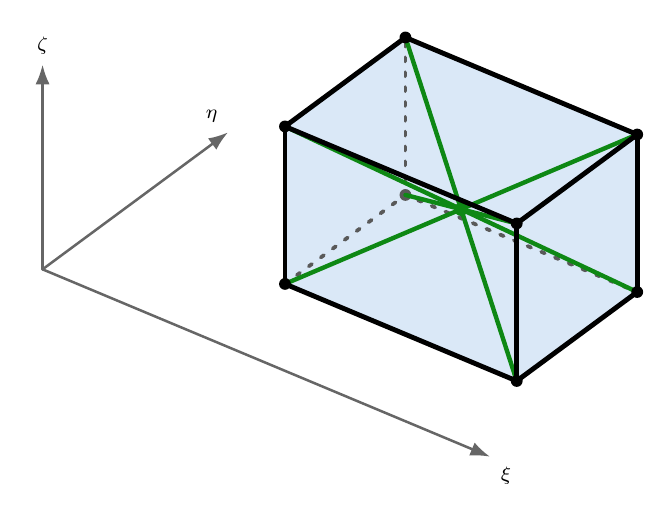
\begin{tikzpicture}[
  x={(20.3mm,-8.5mm)},
  y={(15.3mm,11.3mm)},
  z={(0mm,20mm)},
  line join=round,
  line cap=round,
  outer/.style={draw=black,line width=0.62mm},
  hidden/.style={draw=black!65,line width=0.48mm,loosely dotted},
  face/.style={fill=externalface,fill opacity=0.18,draw=none},
  centroidedge/.style={draw=centroidgreen,line width=0.56mm},
  axis/.style={draw=black!60,line width=0.32mm,-{Latex[length=2.5mm,width=1.8mm]}}
]
  % Hexahedron vertices. The xi direction is stretched to match the prism figures.
  \coordinate (A) at (0,0,0);
  \coordinate (B) at (1.45,0,0);
  \coordinate (C) at (1.45,1,0);
  \coordinate (D) at (0,1,0);
  \coordinate (E) at (0,0,1);
  \coordinate (F) at (1.45,0,1);
  \coordinate (G) at (1.45,1,1);
  \coordinate (H) at (0,1,1);
  \coordinate (center) at (0.725,0.5,0.5);

  % Offset computational-coordinate axes.
  \coordinate (Oaxis) at (-1.20,-0.42,-0.18);
  \draw[axis] (Oaxis) -- (1.60,-0.42,-0.18) node[below right,font=\scriptsize] {$\xi$};
  \draw[axis] (Oaxis) -- (-1.20,1.12,-0.18) node[above left,font=\scriptsize] {$\eta$};
  \draw[axis] (Oaxis) -- (-1.20,-0.42,1.12) node[above,font=\scriptsize] {$\zeta$};

  % Exterior faces remain faint so the centroid-to-vertex split is legible.
  \path[face] (A) -- (B) -- (C) -- (D) -- cycle;
  \path[face] (E) -- (F) -- (G) -- (H) -- cycle;
  \path[face] (A) -- (B) -- (F) -- (E) -- cycle;
  \path[face] (B) -- (C) -- (G) -- (F) -- cycle;
  \path[face] (C) -- (D) -- (H) -- (G) -- cycle;
  \path[face] (D) -- (A) -- (E) -- (H) -- cycle;

  % Hidden geometry is drawn before the centroid split.
  \draw[hidden] (A) -- (D) -- (C);
  \draw[hidden] (D) -- (H);
  \fill[black!65] (D) circle[radius=0.75mm];

  % Cell-based refinement: the element centroid connects to original vertices.
  \foreach \p in {A,B,C,D,E,F,G,H} {
    \draw[centroidedge] (center) -- (\p);
  }
  \fill[centroidgreen] (center) circle[radius=0.86mm];

  % Visible exterior wireframe occludes the centroid split where appropriate.
  \draw[outer] (A) -- (B) -- (C);
  \draw[outer] (E) -- (F) -- (G) -- (H) -- cycle;
  \draw[outer] (A) -- (E);
  \draw[outer] (B) -- (F);
  \draw[outer] (C) -- (G);

  % Visible original vertices are black.
  \foreach \p in {A,B,C,E,F,G,H} {
    \fill[black] (\p) circle[radius=0.75mm];
  }
\end{tikzpicture}
\end{document}
